\documentclass{article}

\usepackage[utf8]{inputenc}
% \usepackage[utf8]{inputenc}
\usepackage{multicol}
\usepackage{dcolumn}
\usepackage[a4paper,top=3cm,bottom=3cm,left=1.5cm,right=1.5cm,marginparwidth=1.75cm]{geometry}
\usepackage{multicol}
\setlength{\columnsep}{0.5cm}
\usepackage{multirow}
\usepackage{amsmath}
\usepackage{graphicx}
\usepackage{hyperref}
\hypersetup{colorlinks=true,linkcolor=blue,filecolor=magenta,urlcolor=cyan,}
\usepackage{amsfonts}
\usepackage{mathtools}
\usepackage{lipsum}
\usepackage{float}
\usepackage{layout}
\usepackage{bm}

\usepackage{listings}
\usepackage{xcolor}
\definecolor{codegreen}{rgb}{0,0.6,0}
\definecolor{codegray}{rgb}{0.5,0.5,0.5}
\definecolor{codepurple}{rgb}{0.58,0,0.82}
\definecolor{backcolour}{rgb}{0.95,0.95,0.92}
\lstdefinestyle{mystyle}{
    backgroundcolor=\color{backcolour},
    commentstyle=\color{codegreen},
    keywordstyle=\color{blue},
    numberstyle=\tiny\color{codegray},
    stringstyle=\color{codepurple},
    basicstyle=\ttfamily\footnotesize,
    breakatwhitespace=false,
    breaklines=true,
    captionpos=b,
    keepspaces=true,
    numbers=left,
    numbersep=5pt,
    showspaces=false,
    showstringspaces=false,
    showtabs=false,
    tabsize=2
}
\lstset{style=mystyle}





\begin{document}










%TitlePage%TitlePage%TitlePage%TitlePage%TitlePage%TitlePage%TitlePage%TitlePage%TitlePage%TitlePage%TitlePage%TitlePage%TitlePage
\thispagestyle{empty}
\baselineskip25pt
\begin{center}
{\Large {\textbf{CALCULATION OF MUON LIFE TIME USING SCINTILLATION \\AND CHERENKOV RADIATION WITH TEACHSPIN SETUP}}}\\
\end{center}

\vfill
\baselineskip15pt
\begin{center}
{\em Open Lab Report Submitted} \\
in Partial Fulfilment of the Requirements \\
for the course \
\vskip .30\baselineskip
{\large{\bf P442-Integrated Laboratory-II}}
\end{center}
\baselineskip25pt

\vfill
\begin{center} {\bf {\em by}} \\
{\large{\bf ANANTHA PADMANABHAN M NAIR}} \\
Course Instructors:\\
\textbf{Dr. Ashok Mohapatra\\
Dr. Gunda Santosh Babu}
\end{center}

\vfill
\begin{center}
\begin{figure}[h!]
\centering

\includegraphics[scale=0.2]{Images/logo1.jpg}
\end{figure}
 {\bf {\em to the }} \\
{\bf {\large School of Physical Sciences}} \\
{\bf {\large National Institute of Science Education and Research}} \\
{\bf Bhubaneswar} \\
{\bf \today} 
\end{center}
%TitlePage%TitlePage%TitlePage%TitlePage%TitlePage%TitlePage%TitlePage%TitlePage%TitlePage%TitlePage%TitlePage%TitlePage%TitlePage%










%Content Table Page%Content Table Page%Content Table Page%Content Table Page%Content Table Page%Content Table Page
\pagenumbering{roman}
\newpage
\newgeometry{top=2.5cm,bottom=2.5cm,left=3.5cm,right=3.5cm}
\begin{center}
 \tableofcontents  
 \newpage
 \listoffigures
 \listoftables 
\end{center}
\restoregeometry
%Content Table Page%Content Table Page%Content Table Page%Content Table Page%Content Table Page%Content Table Page



\newpage
\begin{center}
    \large{\textbf{CALCULATION OF MUON LIFE TIME USING SCINTILLATOR DETECTOR \\ AND CHERENKOV RADIATION WITH TEACHSPIN SETUP}}
\end{center}
\begin{abstract}
    This experiment aimed to determine the mean life of muons using the teachspin setup. Initially, data was collected with a scintillation detector connected to a PMT using teachspin software. Later, the setup was modified, replacing the scintillation detector with a Cherenkov detector connected to the PMT. Data was collected using the same software, and the mean muon life was calculated from this data. Subsequently, both sets of data were analyzed using Python and ROOT libraries. Additionally, a Geant4 simulation was conducted for the modified setup, and its data was also analyzed using ROOT libraries. A comparison was made between the results obtained from the Geant4 simulation and the teachspin setup, followed by a discussion of the findings.
\end{abstract}
\begin{multicols}{2}
\pagenumbering{arabic}






\section{\label{intro}Introduction}
Muon decay experiments have a rich history dating back to the mid-20th century when pioneering physicists first began studying these elusive subatomic particles. Muons, which are heavier cousins of electrons, are known for their fleeting existence, making them fascinating subjects of study in particle physics. Their relatively short lifespan, coupled with their ability to penetrate matter, has led to a myriad of experimental investigations aimed at understanding fundamental aspects of particle physics.

Over the years, muon decay experiments have played a crucial role in advancing our understanding of the Standard Model of particle physics, providing valuable insights into the nature of fundamental particles and their interactions. These experiments have not only contributed to our knowledge of particle physics but have also found practical applications in various fields, including astrophysics, cosmology, and even archaeology.
%%%%%%%%%%%%%%%%%%%%%%%%%%%%%%%%%%%%%%%%%%%%%%%%%%%%%%%%%%%%%%%%%%%%%%%%%%%%%%%%%%%%%%%%%%%%%%%%%%%%%%%%%%%%%%%%%%%%%%%%%%%%%%%%%%%%%%%%%%%%%%%%%%%%%%%%%%
\section{\label{theory}Theory}
Muons are elementary particles similar to electrons but with a much greater mass, making them key players in the study of particle physics. They are classified as leptons, belonging to the same family as electrons and neutrinos. Muons are unstable, with a mean lifetime of around 2.2 microseconds, and they decay into lighter particles, predominantly electrons and neutrinos, through weak interactions. Despite their short lifespan, muons are abundant in cosmic rays and are also produced in particle accelerators, providing ample opportunities for experimental study. 

\subsection{Cosmic Muons}
The muons are primarily generated by the interactions of cosmic rays with the atmospheric particles. The cosmic rays are high-energy particles originating from outer space, which interact with the Earth's atmosphere, producing a cascade of secondary particles, including muons. 

\subsubsection{Cosmic Rays}
Cosmic rays are high-energy particles that originate from various sources beyond our solar system, such as distant stars, supernovae, and active galactic nuclei. They consist of  protons(87\%),Alpha Particles(12\%), and atomic Heavy Nuclei (1\%), some of which can have energies millions or even billions of times greater than those produced in the most powerful particle accelerators on Earth. When  cosmic rays enter the Earth's atmosphere, they interact with air molecules, producing a cascade  of secondary particles, including muons, neutrinos, and gamma rays.

\subsection{Muon Production}

When there Cosmic Rays Reach the Earths atmosphere, it collides with the air molecules and produces 
many particles, mostly Pions and Kaons. These are the primary Particles. These particles then decay to produce a wide variety
of particles most of which are muons. Also, more than 90\% of the cosmic muons are produced from Pions.

From the Kaons, We can see that the muons are produced by the weak interactions and it also produces neutrinos given by:
\begin{equation}
    K^{+} \longrightarrow \mu^{+} + \nu_{\mu}
\end{equation}

From the decay of Pions, 64\% of the time, disintegrates directly into $\mu^+$; 21\% of the time into $\pi^0$and$\pi^+$ and Only 6\% of the disintegrations produce three particles-$\mu^+$,$\mu^+$,$\mu-$. These pions then decay to produce muons according to:
\begin{equation}
    \pi^{+} \longrightarrow \mu^{+} + \nu_{\mu}
\end{equation}
\begin{equation}
    \pi^{-} \longrightarrow \mu^{-} + \Bar{\nu_{\mu}}
\end{equation}



While the decay of these primary particles produces mostly muons, Many other elementary particles are also produced
within this process. During the process of generation of primary particles that is the Kaons and pions, $K^0$ and $\pi^0$ are also produced
which on decay produces $\gamma$-particles. These Muons and other particles further decay to produce Electrons and Positrons.





\subsection{Muon Properties}

Muons are unstable particles having intermediate mass between that of an 
electron and a proton, just like charged pions. Compared to pions, they are 
a little lighter.The muons carry one unit of electrical charge, either positive 
or negative, and are electrically charged. The life time of the muon is $2.2\mu s$.
The properties of the muons are tabulated below in Table-\ref{muonproperty}

\begin{table}[H]
    \centering
    \resizebox{0.85\columnwidth}{!}{%
    \begin{tabular}{|cc|c|}
        \hline
        \multicolumn{2}{|c|}{\textbf{Properties}}                           & \textbf{Values}              \\ \hline
        \multicolumn{1}{|c|}{\multirow{2}{*}{\textbf{Mass}}} & $m_{\mu}$    & $206.7686m_e$                \\ \cline{2-3} 
        \multicolumn{1}{|c|}{}                               & $m_{\mu}c^2$ & 105.659MeV                   \\ \hline
        \multicolumn{1}{|c|}{\textbf{Mean Life}}             & $\tau_{\mu}$ & $2.197 \mu s$                \\ \hline
        \multicolumn{1}{|c|}{\textbf{Spin}}                  & $s_{\mu}$    & 1/2                          \\ \hline
        \multicolumn{1}{|c|}{\textbf{Magnetic   Moment}}     & $\mu_{\mu}$  & $\frac{eh}{4\pi   m_{\mu} }$ \\ \hline
    \end{tabular}%
    }
    \caption{Properties of Muons}
    \label{muonproperty}
\end{table}



\subsection{Life time of Muons at Relativistic Speeds}

We know that the average energy of the cosmic muons are $4GeV$, which, for a particle of mass $m_{\mu}$, is a relativistic speed. The life time of the muon at rest is $2.2\mu s$. But when the muon is moving at relativistic speeds (with respect to the observer on earth), the life time of the muon is given by the formula:
\begin{equation}
    \tau = \frac{\tau_{0}}{\sqrt{1-\frac{v^2}{c^2}}}
\end{equation}

Where $\tau_{0}$ is the life time of the muon at rest, $v$ is the velocity of the muon and $c$ is the speed of light. In order to calculate the $\gamma$ factor, we can use the formula:
\begin{equation}
    E_{total} = 4GeV = \gamma m_{\mu}c^2
\end{equation}

From this, we can calculate the $\gamma$ factor and then calculate the life time of the muon at relativistic speeds. The gamma came out to be 38.1 and the life time of the muon at relativistic speeds is $ 84 \mu s$ which is more than eneoygh time for the high energy muons to reach the earths surface.


\subsection{Decay of Muons}

These Muons decay into electrons and neutrinos through the weak interactions. The decay of the muon is given by:
\begin{equation}
    \mu^{-} \longrightarrow e^{-} + \Bar{\nu_{e}} + \nu_{\mu}
\end{equation}
and for the muon decay into positron, the decay is given by:
\begin{equation}
    \mu^{+} \longrightarrow e^{+} + \nu_{e} + \Bar{\nu_{\mu}}
\end{equation}


The decay of the muon in the scintillation detector occurs when the muon comes to a complete stop inside the detector. This muon spends some time in the order of micro seconds inside the detector before decaying into electrons and neutrinos. After coming to rest, the muons only energy is its mass energy $m_\mu c^2$ whih gets converted to the kinetic energy of the electrons and neutrinos. The electrons and neutrinos are produced with a wide range of energies, but the average energy of the electrons is $35 MeV$(The two neutrinos, $\nu$, carry away the rest of the energy undetectably.). This electron has eneough energy to excite the scintillator material and produce light. So, we will get 2 pulses from the scintillator, one due to the muon stopping and the other due to the decay of the muon.


Indeed, the distribution decaying over time should follow an exponential pattern, representing the 'survival curve' of muons. This curve won't depict the muons' survival time since their inception in the upper atmosphere, but rather their survival time since reaching the scintillator.

So, we can get the mean life by fitting the distribution of the decay times of the muons in the scintillator detector. The fitting function is given by:
\begin{equation}
    N(t) = N_0 e^{-t/\tau} + B
\end{equation}
Where $N(t)$ is the number of muons decaying at time $t$, $N_0$ is the number of muons decaying at time $t=0$, $\tau$ is the mean life of the muon and $B$ is the background noise. The mean life of the muon can be calculated by fitting the distribution of the decay times of the muons in the scintillator detector.


Now, from the calculations from previous subsection, the time required for the muon to reach the scintillator detector is approximately $200 \mu s$. 




The fraction of the muons that survive to get to the scintillator detector is given by:
\begin{equation}
    f = e^{-(t=200 \mu s /(\gamma = 40) )/(\tau = 2 \mu s)} = e^{-5/2}
\end{equation}
which is approximately 10\% od the total muons.
So we will be able to detect approximately 10\% of all the muons that enter the earth with a flux of $1$ per $cm^2$ per second.




\subsection{Cherenkov Radiation}

Cherenkov radiation is a phenomenon that occurs when a charged particle passes through a dielectric medium at a speed greater than the phase velocity of light in that medium. As the particle moves through the medium, it polarizes the atoms or molecules, causing them to emit electromagnetic radiation in the form of photons. This emitted radiation is known as Cherenkov radiation. It appears as a cone of light with a characteristic blue color, and its intensity and angle of emission depend on the velocity and charge of the particle. 


The light emitted from the process forms a cone inside the radiator. The angle of the cone is given by:
\begin{equation}
    \cos(\theta) = \frac{1}{\beta n}
\end{equation}


Where n is the refractive index of the medium and $\beta$ is the velocity of the particle in units of the speed of light.

The illustration of the Cherenkov radiation is shown in the figure-\ref{cherenkov}.

\begin{figure}[H]
    \centering
    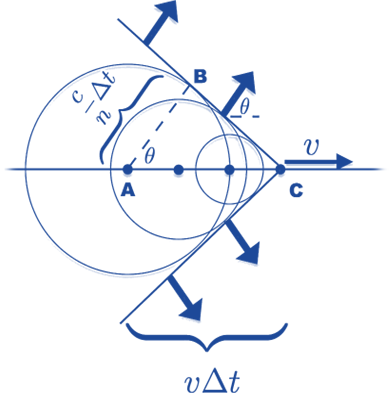
\includegraphics[scale=0.5]{Images/cherenkovcone.png}
    \caption{Illustration of Cherenkov Radiation}
    \label{cherenkov}
\end{figure}



\subsection{Fermi Coupling Constant}

The Fermi constant is a measure of the strength of the weak force.  Its measurement is $1.435 \times 10^{-36}J/m^3$. Measurements of the muon lifetime, which are inversely proportional to the square of GF (when ignoring the muon mass against the mass of the W boson) provide the most accurate experimental estimate of the Fermi coupling constant. The relationship between the muon lifetime $\tau$ and GF is expressed by the following equation:
 \begin{equation}
     \tau=\frac{192*\pi^3*\hbar^7}{G_f^2*m_\mu^5*c^4}
 \end{equation}
where, $\tau$ is the mean lifetime of the muon, GF is the Fermi coupling constant, $m_\mu$ is the mass of the muon and, c is the speed of light.
\subsection{GEANT4 Toolkit}
Geant4 is a toolkit for the simulation of the passage of particles through matter. Using Geant4 tool, we have simulated both of our experiments and compared the results.






\subsection{Geant4 Simulations}

Geant4 is a powerful toolkit developed by CERN for simulating the passage of particles through matter. Widely used in various fields including high-energy physics, medical physics, and space science, Geant4 offers a comprehensive set of functionalities for modeling complex geometries, particle interactions, and detector responses. Its versatility allows researchers to simulate a wide range of experimental setups accurately, aiding in the design, optimization, and analysis of experiments. With its open-source nature and continuous development, Geant4 remains at the forefront of particle transport simulations, facilitating groundbreaking discoveries and advancements in numerous scientific disciplines.

The Simulations with an almost same geometry as that is present in the lab has been done in the Geant4 and compared with the results obtained from the teachspin setup. The Geant4 simulations were done with the same geometry as that of the teachspin setup and the data was analyzed using the ROOT libraries.This is done for both the setup with the old scintillator detector and the new Cherenkov detector.

The simulation of the cosmic muons and showers has been done using the EcoMug Standalone header file in C/C++. The Whole software is based on Monte Carlo Simulations and the data obtained from the simulations are analyzed using the ROOT libraries. The data obtained from the simulations are compared with the data obtained from the teachspin setup and the results are discussed in the later sections.
%%%%%%%%%%%%%%%%%%%%%%%%%%%%%%%%%%%%%%%%%%%%%%%%%%%%%%%%%%%%%%%%%%%%%%%%%%%%%
%%%%%%%%%%%%%%%%%%%%%%%%%%%%%%%%%%%%%%%%%%%%%%%%%%%%%%%%%%%%%%%%%%%%%%%%%%%%%
\section{\label{expsetup}Experimental Setup and Procedure }

In the Setup of the Experiment, we have used two methods of detection of the muons. One is with the scintillator detector and the other is with the Cherenkov detector. The Setup with the scitillation is already built and we just had to use the Teachspin set up and the software provided by them to collect the data. The setup with the Cherenkov detector is built by us and the data is collected using the same Teachspin software.

\subsection{Scintillation Detector}

The Scintillation detector that we used consist of a large block of Plasric Sciltillator of Size $26.5cm \times 15cm \times 26.5cm$. This Detector is covered with a white reflective surface which is then covered with a black tape to prevent the light from escaping. The Photomultiplier tube is placed at the top of the detector and is connected to the computer using a USB cable. A high voltage supply is connected to the PMT to provide the necessary voltage for the PMT to work.

\subsection{Photomultiplier Tube}

The Photomultiplier tube is a device that converts the light produced by the scintillator into an electrical signal. The PMT consists of a photocathode, a series of dynodes, and an anode. When a photon strikes the photocathode, it releases an electron, which is then accelerated towards the first dynode. The electron is multiplied at each dynode, resulting in a cascade of electrons that are collected at the anode, producing an electrical signal proportional to the intensity of the light.
The working of the scintillator tube is shown in the figure-\ref{pmt}.
\begin{figure}[H]
    \centering
    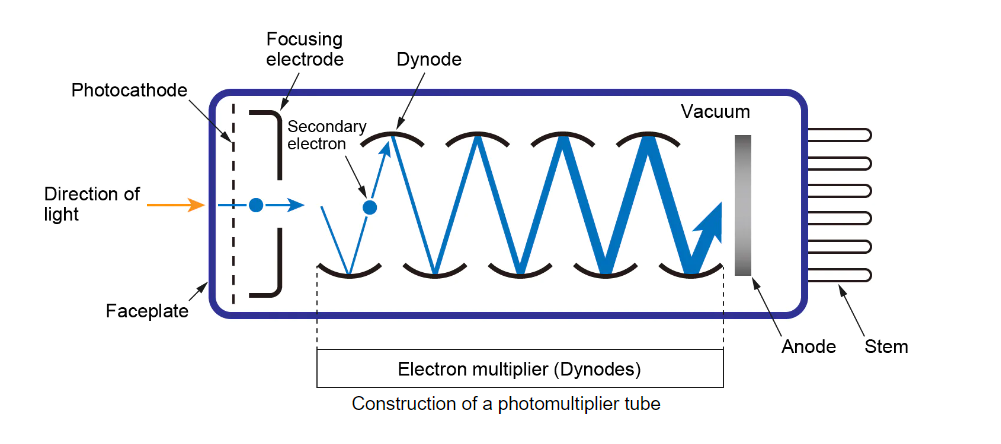
\includegraphics[width = \columnwidth]{Images/pmtsetup.png}
    \caption{Illustration of the working of the Photomultiplier Tube.source:}
    \label{pmt}
\end{figure}

The setup of the scintillator along with the PMT is shown in the figure-\ref{scintsetup}.

\begin{figure}[H]
    \centering
    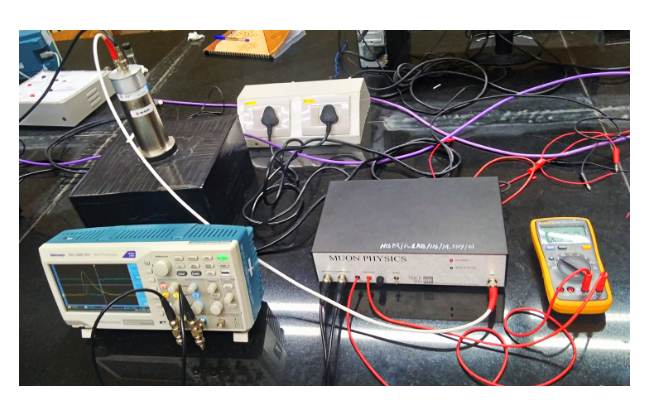
\includegraphics[width = \columnwidth]{Images/scintsetup.png}
    \caption{Setup of the experiment that uses the scintillator detector.}
    \label{scintsetup}
\end{figure}


\subsection{The Teachspin Setup}
The complete instrument has three hardware components: a detector, readout electronics and user-supplied personal computer (PC). Control and data acquisition software are also included.

The output from the PMT is fed into a 2 stage amplifier circuit, which amplifies the signal so that it has sufficient voltage to be considered as a signal by the discriminator. We feed the signal from the amplifier to a discriminator circuit, which has a threshold voltage. The number
of muon readings decreases with increase with threshold
voltage since it reject pulses below the specified threshold level. Since the PMT signal is in the negative region, the discriminator voltage applied is also negative.

The circuit diagram for the teachspin setup is shoen in the figure-\ref{circuit}.
\begin{figure}[H]
    \centering
    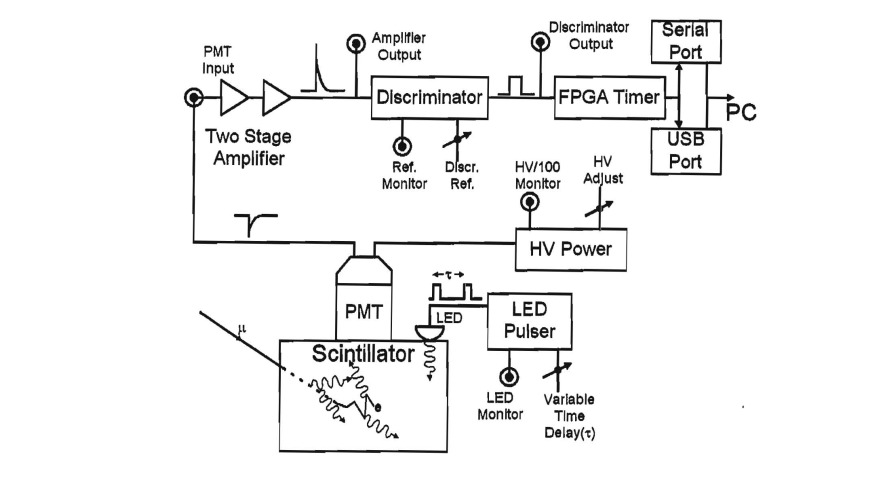
\includegraphics[width = \columnwidth]{Images/circuit.png}
    \caption{The circuit diagram of the teachspin setup.}
    \label{circuit}
\end{figure}

\subsection{The Cherenkov Detector}

In this part we replaced the scintillator with a cherenkov radiator. The Cherenkov radiator in our experiment was distilled water. For the setup we have brought a milton flask with a reflective coating inside. The PMT is placed at the top of the flask and the flask is filled with distilled water. The PMT is connected to the computer using a USB cable and the high voltage supply is connected to the PMT to provide the necessary voltage for the PMT to work. The PMT is then connected to computer via the Teachspin setup to collect the data. The setup that we made is shown in the figure-\ref{cherenkovsetup}.


\begin{figure}[H]
    \centering
    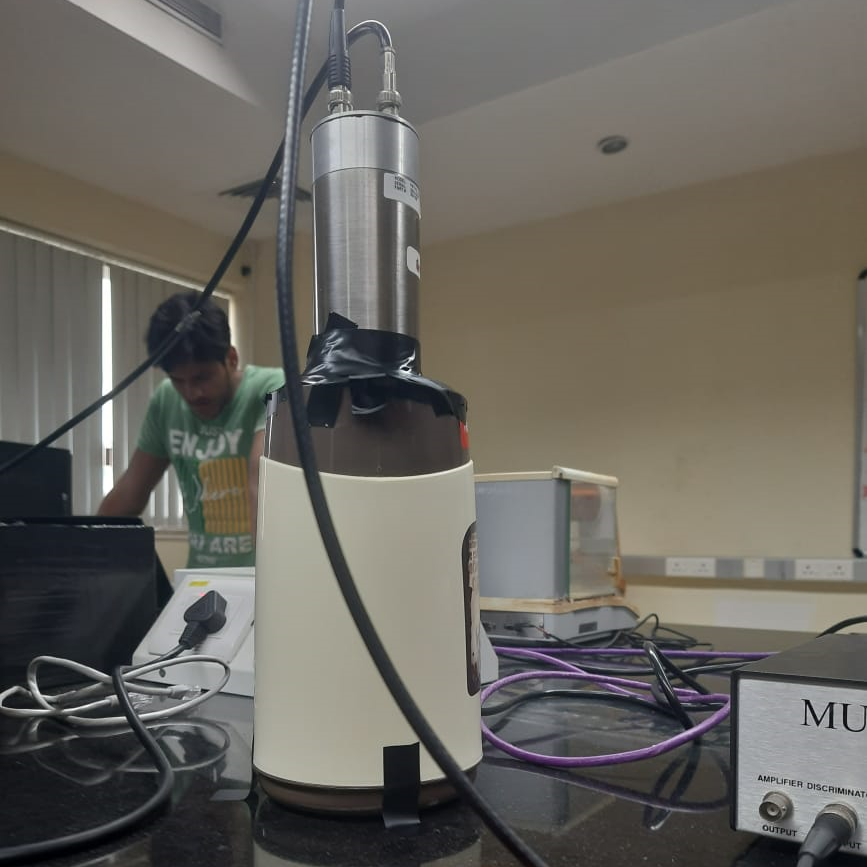
\includegraphics[width = \columnwidth]{Images/cherenkovsetup.png}
    \caption{The modified setup of the experiment that uses the Cherenkov detector.}
    \label{cherenkovsetup}
\end{figure}


\subsection{The Procedure and the Working of the Setups}

In both the setups the working of the setup is the same. The cosmic muons enter the detector and the PMT detects the light produced by the scintillator or the Cherenkov radiator. The PMT converts the light into an electrical signal which is then fed into the computer. The computer records the time at which the muon enters the detector and the time at which the muon decays.

The measureent of the time of decay is done by triggering the timers present in the Teachspin setup. When a high energy muon enters the scintillator/cherenkov a light cone is produced. It uis detected by the PMT which produces a signal. This signal triggers a timer and it starts the timer. There are two reasons for the timer to stop:
\begin{enumerate}
    \item The muon decays and the light produced by the decay is detected by the PMT. This signal stops the timer.
    \item If there is no signal for 40 microseconds. The timer automatically stops.
\end{enumerate}

In the 1st case. The time is registered and is filled into a histogram . if the timer reaches the mark of 40 microseconds, the timer stops and the time is not registered. This is done to prevent the registering of another muon that may enter the detector and creates random signals.
Also, the probability of 2 muons enetering the detector within this 200 microsecond time frame is very low. So, for very large number of data points, we can see safely ignore the case where a second muon stops the timer. Its been calculated that the average time interval between two muons is 200 microseconds.

%%%%%%%%%%%%%%%%%%%%%%%%%%%%%%%%%%%%%%%%%%%%%%%%%%%%%%%%%%%%%%%%%%%%%%%%%%%%%
\section{\label{simobs}Performance and Geometry Simulations using Geant4}

The exact geometry of the setup that is present in the lab is simutaled in the Geant4. The room in which we were doing the Experiment has a size of $7.62m\times\times 3.048m \times 9.144m$. This is set as the world volume for both the simulation of the scintillator and the cherenlov setup. In both the cases the the PMT and the setup is approximated to be placed in the center of the room which is the world Volume. The scintillator is approximated to be a block of plastic scintillator of size $26.5cm \times 15cm \times 26.5cm$ and the Cherenkov radiator is a volume of water in the shape of a cylinder with radius of 4cm and height of 17cm. The reflectivity of the inner surface fr both of the setup is taken to be 0.7. The outer casing of the PMT is taken to be Aluminium. It is a cylinder of diameter 8.5 cm and height of 12cm. The geometry of the scintillator setup is shown in the figure-\ref{scintgeo} and the geometry of the cherenkov setup is shown in the figure-\ref{chergeo}.


\begin{figure}[H]
    \centering
    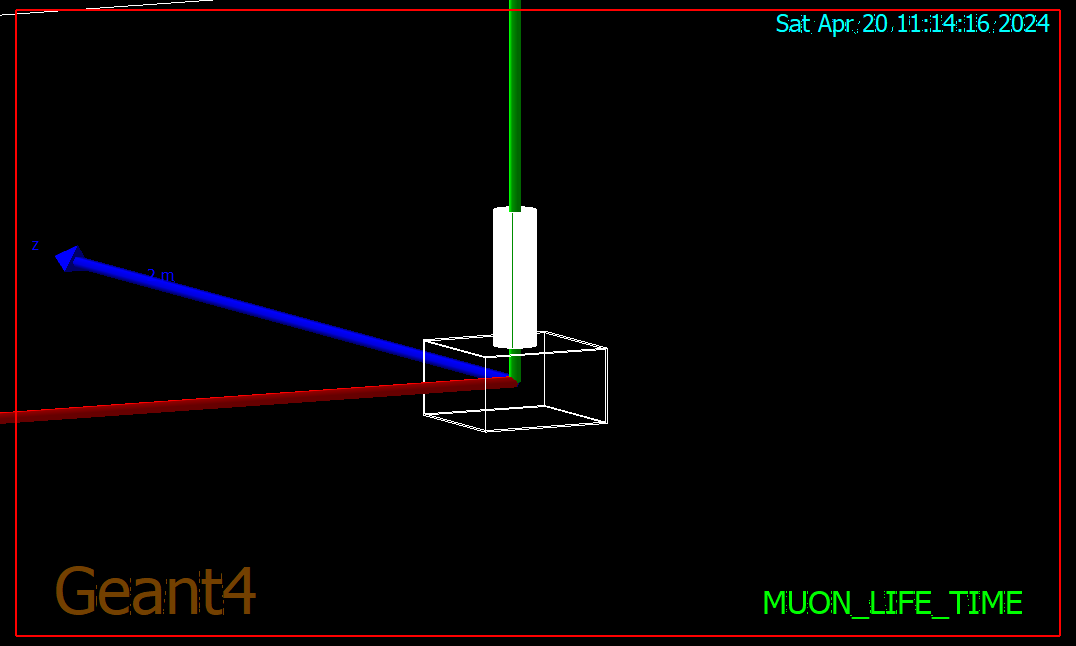
\includegraphics[width = \columnwidth]{Images/scint_sim_1.png}
    \caption{The Simulation geometry of the scintillator detector.}
    \label{scintgeo}
\end{figure}


\begin{figure}[H]
    \centering
    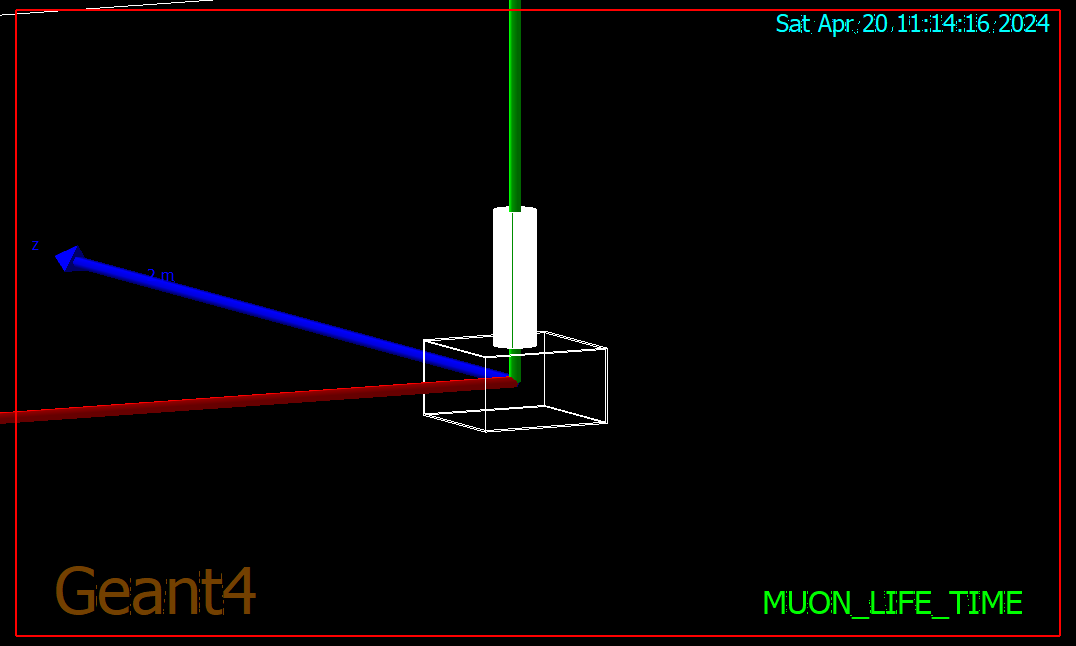
\includegraphics[width = \columnwidth]{Images/scint_sim_1.png}
    \caption{The Simulation geometry of the Cherenkov radiator}
    \label{chergeo}
\end{figure}

The simulation of the cosic muons and showers are simulated by the EcoMug Standalone header file in C/C++. The data obtained, that is momentum and initial position of the muons are give an input to the ParticleGun of the Geant4 and the 100000 runs are made. Since it takes a lot of GPU power to render the simulation image of 100000 runs. A single run for demonstration is shown in the figure-\ref{sim_run}.

\begin{figure}[H]
    \centering
    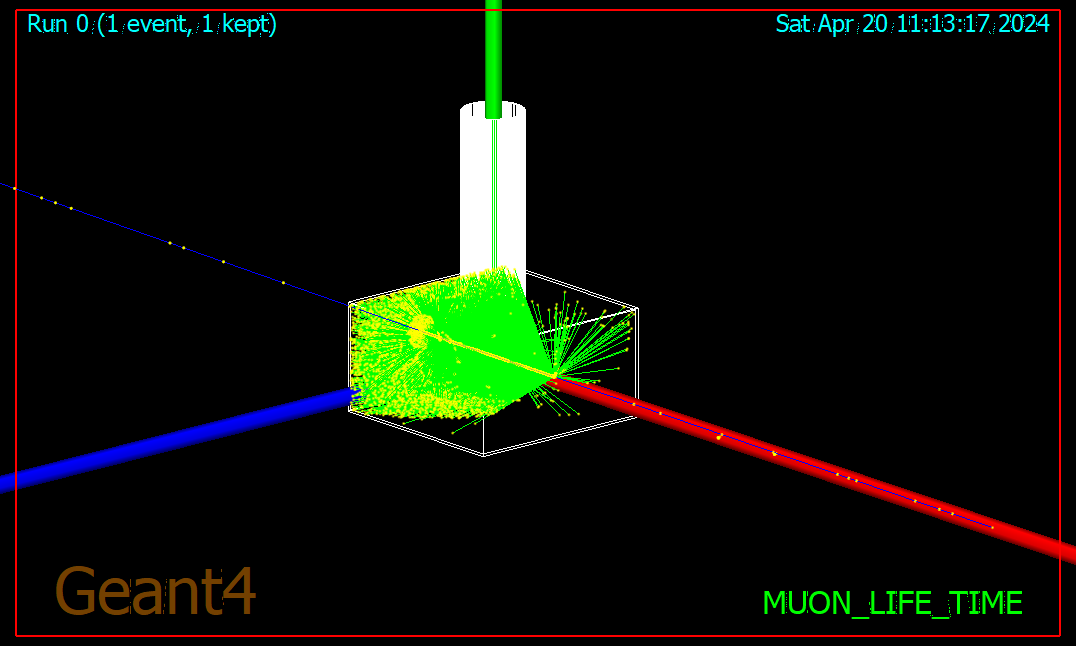
\includegraphics[width = \columnwidth]{Images/scint_sim_2.png}
    \caption{The production of the light cone in the scintillator due to the cosmic muons and its decay. Here the Blue line represents the cosmic muon plus and the green lines represent the optical photons created in the scintillator. in the 3D image the decayed Electron can also be observed.}
    \label{sim_run}
\end{figure}


In the simulations, the main aim was to compare the muon flux for both the detectors. 


%%%%%%%%%%%%%%%%%%%%%%%%%%%%%%%%%%%%%%%%%%%%%%%%%%%%%%%%%%%%%%%%%%%%%%%%%%%%%
%%%%%%%%%%%%%%%%%%%%%%%%%%%%%%%%%%%%%%%%%%%%%%%%%%%%%%%%%%%%%%%%%%%%%%%%%%%%%
\section{\label{observations}Observations and Data}

In this section, we will discuss about the collected data using the scintillator and the Cherenkov detector. Using the Scintillator setup, we took data with different Operating vltages and different threshold voltages.


\subsection{Data from the Scintillator Detector}
The collected data for the scintilation detector is fit in python-\cite{python} and ROOT-\cite{ROOT} to get the mean life of the muons. The plot of the fitted histogram is shown in the figure-\ref{scintplots}. The data for each of these readings are taken for a time period of 1 day each.
\begin{figure*}
    \centering
    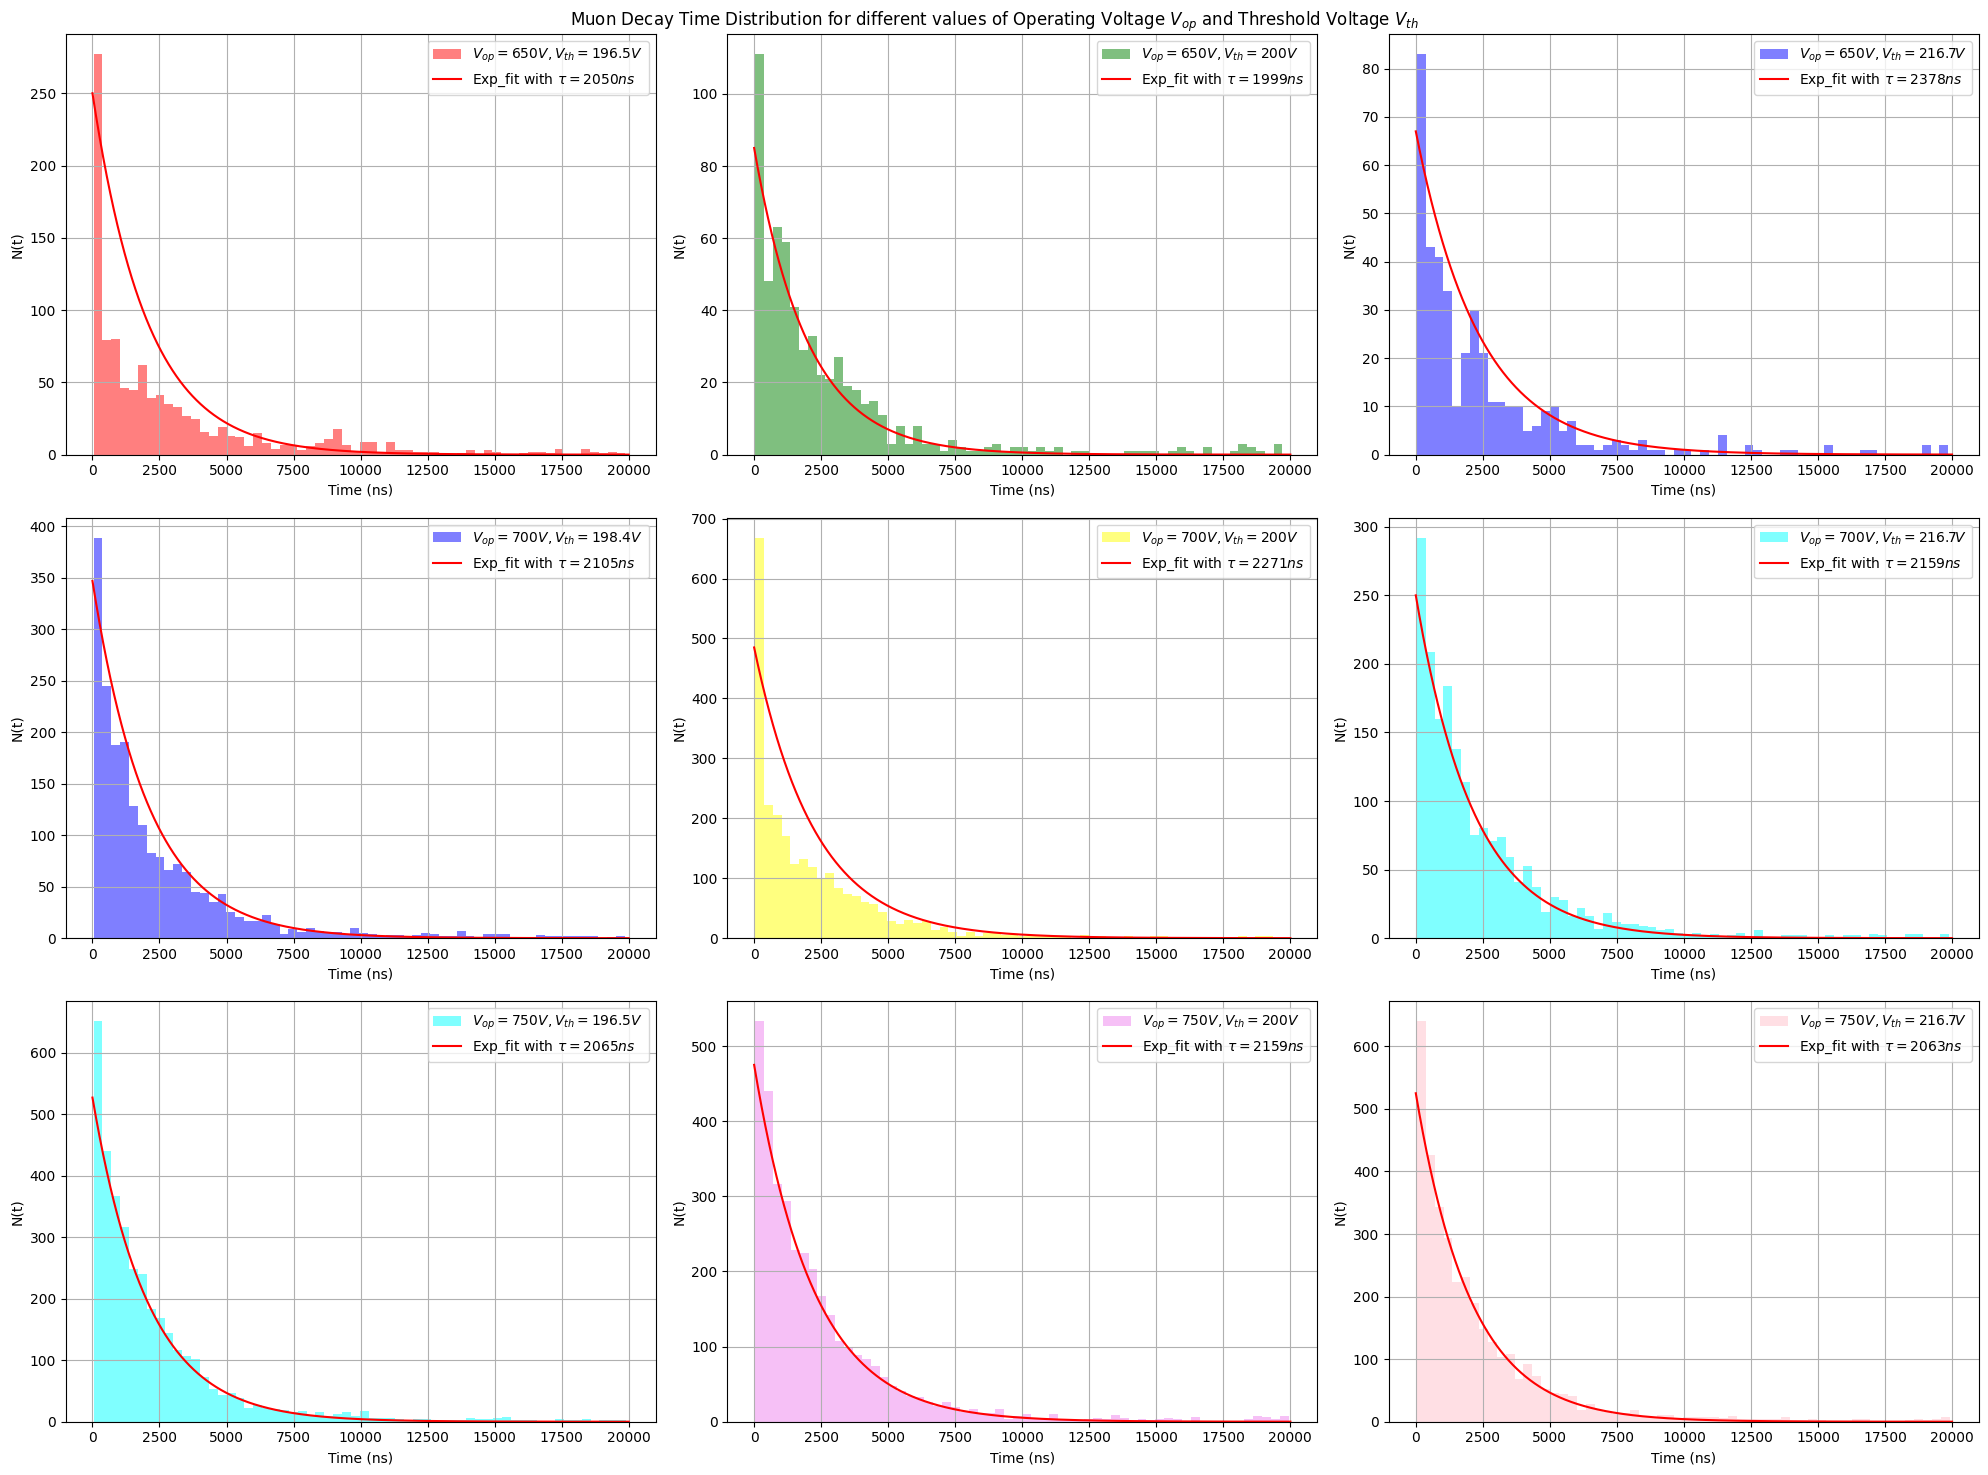
\includegraphics[width = 2\columnwidth]{Images/scint_plots.png}
    \caption{THe fitted plots of the data collected using the scintillator detector.}
    \label{scintplots}
\end{figure*}

\subsection{Data from the Cherenkov Detector}

Due to lack of time, we couldnot get eneough data for the confirmation of the muon detection. Only one set of Data is taken with an operating voltage of 750V and a threshold voltage of 100mV. The data is shown in the figure-\ref{cherenkovplot}. The data was taken for a tim duration of approximately 75 hours. 
\begin{figure}[H]
    \centering
    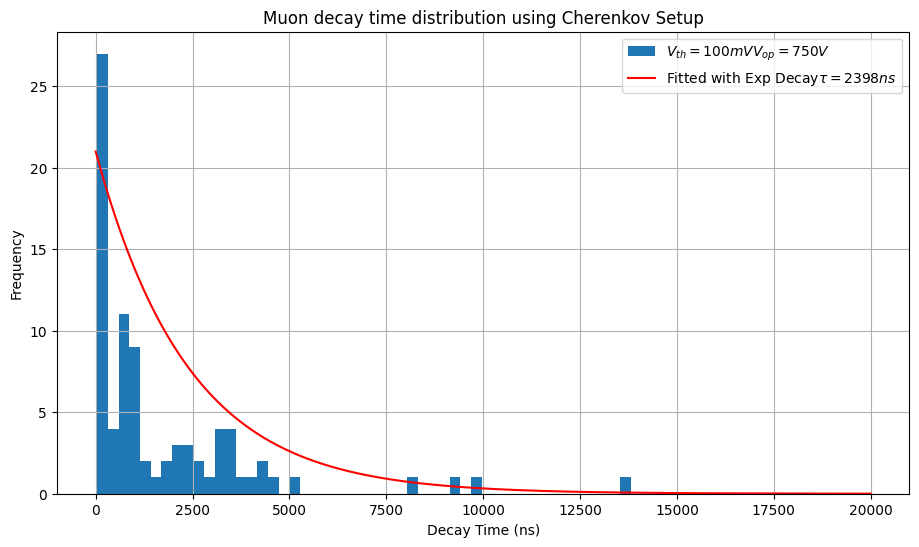
\includegraphics[width = \columnwidth]{Images/cher_plots.png}
    \caption{The fitted plot of the data collected using the cherenkov radiator.-\cite{python}}
    \label{cherenkovplot}
\end{figure}



%%%%%%%%%%%%%%%%%%%%%%%%%%%%%%%%%%%%%%%%%%%%%%%%%%%%%%%%%%%%%%%%%%%%%%%%%%%%%
%%%%%%%%%%%%%%%%%%%%%%%%%%%%%%%%%%%%%%%%%%%%%%%%%%%%%%%%%%%%%%%%%%%%%%%%%%%%%
\section{\label{dataanalysis}Data analysis}


The plots are shown in the previous section. The fitting is done in Python and ROOT. The Results after fitting is tabulated in the table-\ref{scint_res}.


\begin{table*}[h]
    \centering
    \resizebox{2\columnwidth}{!}{%
    \begin{tabular}{|c|ccc|ccc|ccc|}
    \hline
    \multirow{2}{*}{\textbf{Property}} & \multicolumn{3}{c|}{\textbf{$V_{op}   = 650V$}} & \multicolumn{3}{c|}{\textbf{$V_{op}   = 700V$}} & \multicolumn{3}{c|}{\textbf{$V_{op}   = 750V$}} \\ \cline{2-10} 
     & \multicolumn{1}{c|}{\textbf{$V_{th} = 196.5 mV$}} & \multicolumn{1}{c|}{\textbf{$V_{th} = 200mV$}} & \textbf{$V_{th} = 216.7$} & \multicolumn{1}{c|}{\textbf{$V_{th} = 198.4 mV$}} & \multicolumn{1}{c|}{\textbf{$V_{th} = 200mV$}} & \textbf{$V_{th} = 216.7$} & \multicolumn{1}{c|}{\textbf{$V_{th} = 196.5 mV$}} & \multicolumn{1}{c|}{\textbf{$V_{th} = 200mV$}} & \textbf{$V_{th} = 216.7$} \\ \hline
    \textbf{MeanLife (ns)} & \multicolumn{1}{c|}{2050} & \multicolumn{1}{c|}{1999} & 2378 & \multicolumn{1}{c|}{2105} & \multicolumn{1}{c|}{2271} & 2159 & \multicolumn{1}{c|}{2065} & \multicolumn{1}{c|}{2159} & 2063 \\ \hline
    \textbf{Error (ns)} & \multicolumn{1}{c|}{97} & \multicolumn{1}{c|}{112} & 134 & \multicolumn{1}{c|}{77} & \multicolumn{1}{c|}{65} & 59 & \multicolumn{1}{c|}{36} & \multicolumn{1}{c|}{46} & 37 \\ \hline
    \end{tabular}%
    }
    \caption{The results of the fitted data from the Scintillation detector}
    \label{scint_res}
\end{table*}


For the cherenkov radiator, as seen in the figure-\ref{cherenkovplot}
The value of the Muon lifetime is obtained as 2398 ns with an error of 237 ns. The percentage error is 9.8\%.

%%%%%%%%%%%%%%%%%%%%%%%%%%%%%%%%%%%%%%%%%%%%%%%%%%%%%%%%%%%%%%%%%%%%%%%%%%%%%
%%%%%%%%%%%%%%%%%%%%%%%%%%%%%%%%%%%%%%%%%%%%%%%%%%%%%%%%%%%%%%%%%%%%%%%%%%%%%
\section{\label{error}Error Analysis}

From the table-\ref{scint_res}, the error in the mean life of muons calculated from the scintillation detector are far more high at an operating voltage of 650V. So, we will consider the operating voltage as 750V. The error in the mean life of the muons is calculated by taking the average of all the errors.
so the Muon life time is given by:

\begin{equation}
    \tau = 2096 \pm 40 ns
\end{equation}
with a percentage error of 1.9\%.


Now for the 

%%%%%%%%%%%%%%%%%%%%%%%%%%%%%%%%%%%%%%%%%%%%%%%%%%%%%%%%%%%%%%%%%%%%%%%%%%%%%
%%%%%%%%%%%%%%%%%%%%%%%%%%%%%%%%%%%%%%%%%%%%%%%%%%%%%%%%%%%%%%%%%%%%%%%%%%%%%
\section{\label{results}Results}

%%%%%%%%%%%%%%%%%%%%%%%%%%%%%%%%%%%%%%%%%%%%%%%%%%%%%%%%%%%%%%%%%%%%%%%%%%%%%
%%%%%%%%%%%%%%%%%%%%%%%%%%%%%%%%%%%%%%%%%%%%%%%%%%%%%%%%%%%%%%%%%%%%%%%%%%%%%
\section{\label{Conclusion}Conclusion and Discussions}

hihi-\cite{ROOT}
%%%%%%%%%%%%%%%%%%%%%%%%%%%%%%%%%%%%%%%%%%%%%%%%%%%%%%%%%%%%%%%%%%%%%%%%%%%%%
%%%%%%%%%%%%%%%%%%%%%%%%%%%%%%%%%%%%%%%%%%%%%%%%%%%%%%%%%%%%%%%%%%%%%%%%%%%%%

\end{multicols}
\bibliographystyle{plain}
\bibliography{bib.bib}


\end{document}